% Generated by code/needham.py -- do not edit by hand.
\definecolor{qocA}{rgb}{0.00,0.45,0.70}
\definecolor{qocB}{rgb}{0.90,0.60,0.00}
\definecolor{qocC}{rgb}{0.00,0.62,0.45}
\definecolor{qocD}{rgb}{0.80,0.40,0.00}
\definecolor{qocE}{rgb}{0.80,0.60,0.70}
\definecolor{qocF}{rgb}{0.35,0.70,0.90}
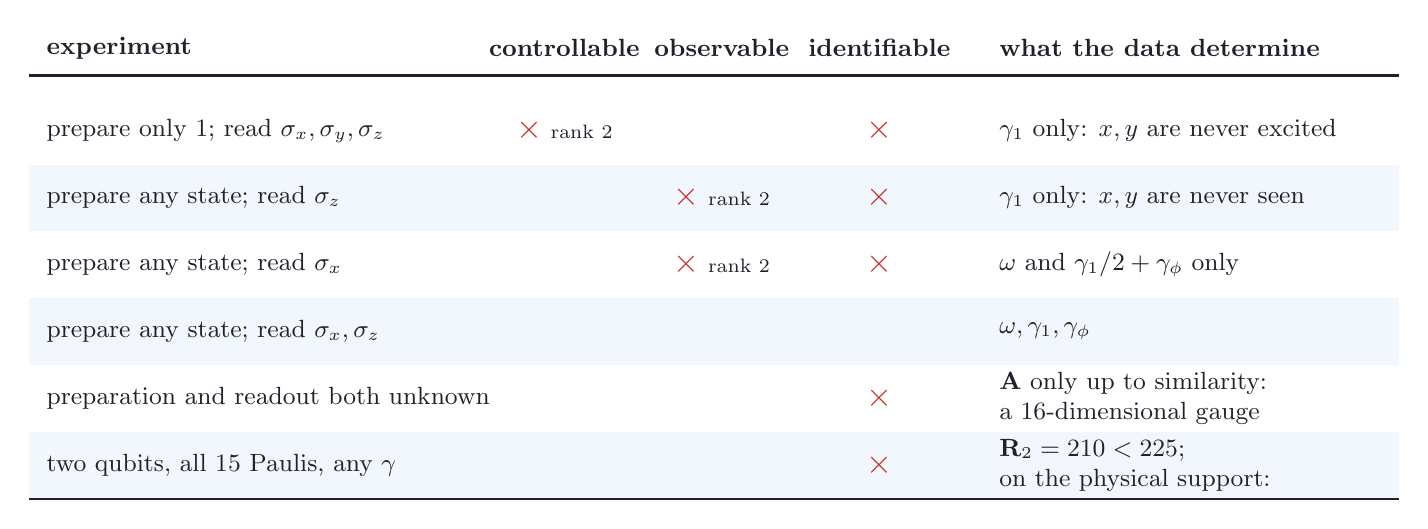
\begin{tikzpicture}[ink/.style={line width=0.9pt, ndInk}, faint/.style={line width=0.4pt, ndInk!35}, dashedink/.style={line width=0.5pt, ndInk!55, dash pattern=on 2.5pt off 2pt}, vec/.style={->, >=stealth, line width=1.2pt}, note/.style={font=\footnotesize\itshape, text=ndInk!85, align=center}, pointer/.style={->, >=stealth, line width=0.4pt, ndInk!60, shorten >=2pt, shorten <=1pt}, dot/.style={circle, fill=ndInk, inner sep=0pt, minimum size=3.4pt}, wash/.style={fill=ndSky, fill opacity=0.55}, every node/.style={text=ndInk}]
\definecolor{ndInk}{rgb}{0.13,0.13,0.18}
\definecolor{ndPaper}{rgb}{0.99,0.96,0.88}
\definecolor{ndSky}{rgb}{0.84,0.91,0.98}
\definecolor{ndRose}{rgb}{0.98,0.86,0.84}
\definecolor{ndBlue}{rgb}{0.13,0.36,0.66}
\definecolor{ndRed}{rgb}{0.78,0.20,0.16}
\definecolor{ndGold}{rgb}{0.88,0.62,0.10}
\definecolor{ndGreen}{rgb}{0.18,0.52,0.30}
\node[anchor=west, font=\small\bfseries] at (0.00,0.6) {experiment};
\node[anchor=center, font=\small\bfseries] at (6.70,0.6) {controllable};
\node[anchor=center, font=\small\bfseries] at (8.70,0.6) {observable};
\node[anchor=center, font=\small\bfseries] at (10.70,0.6) {identifiable};
\node[anchor=west, font=\small\bfseries] at (12.10,0.6) {what the data determine};
\draw[ink] (-0.1,0.25) -- (17.3,0.25);
\node[anchor=west, font=\small] at (0.0,-0.45) {prepare only $\ket1$; read $\sigma_x,\sigma_y,\sigma_z$};
\node[font=\small] at (6.70,-0.45) {\textcolor{ndRed}{\large $\times$}\ {\scriptsize rank $2$}};
\node[font=\small] at (8.70,-0.45) {\textcolor{ndGreen}{\large $\checkmark$}};
\node[font=\small] at (10.70,-0.45) {\textcolor{ndRed}{\large $\times$}};
\node[anchor=west, font=\small, align=left] at (12.1,-0.45) {$\gamma_1$ only: $x,y$ are never excited};
\fill[ndSky, opacity=0.35] (-0.1,-0.88) rectangle (17.3,-1.73);
\node[anchor=west, font=\small] at (0.0,-1.30) {prepare any state; read $\sigma_z$};
\node[font=\small] at (6.70,-1.30) {\textcolor{ndGreen}{\large $\checkmark$}};
\node[font=\small] at (8.70,-1.30) {\textcolor{ndRed}{\large $\times$}\ {\scriptsize rank $2$}};
\node[font=\small] at (10.70,-1.30) {\textcolor{ndRed}{\large $\times$}};
\node[anchor=west, font=\small, align=left] at (12.1,-1.30) {$\gamma_1$ only: $x,y$ are never seen};
\node[anchor=west, font=\small] at (0.0,-2.15) {prepare any state; read $\sigma_x$};
\node[font=\small] at (6.70,-2.15) {\textcolor{ndGreen}{\large $\checkmark$}};
\node[font=\small] at (8.70,-2.15) {\textcolor{ndRed}{\large $\times$}\ {\scriptsize rank $2$}};
\node[font=\small] at (10.70,-2.15) {\textcolor{ndRed}{\large $\times$}};
\node[anchor=west, font=\small, align=left] at (12.1,-2.15) {$\omega$ and $\gamma_1/2+\gamma_\phi$ only};
\fill[ndSky, opacity=0.35] (-0.1,-2.58) rectangle (17.3,-3.43);
\node[anchor=west, font=\small] at (0.0,-3.00) {prepare any state; read $\sigma_x,\sigma_z$};
\node[font=\small] at (6.70,-3.00) {\textcolor{ndGreen}{\large $\checkmark$}};
\node[font=\small] at (8.70,-3.00) {\textcolor{ndGreen}{\large $\checkmark$}};
\node[font=\small] at (10.70,-3.00) {\textcolor{ndGreen}{\large $\checkmark$}};
\node[anchor=west, font=\small, align=left] at (12.1,-3.00) {$\omega,\gamma_1,\gamma_\phi$};
\node[anchor=west, font=\small] at (0.0,-3.85) {preparation and readout both unknown};
\node[font=\small] at (6.70,-3.85) {\textcolor{ndGreen}{\large $\checkmark$}};
\node[font=\small] at (8.70,-3.85) {\textcolor{ndGreen}{\large $\checkmark$}};
\node[font=\small] at (10.70,-3.85) {\textcolor{ndRed}{\large $\times$}};
\node[anchor=west, font=\small, align=left] at (12.1,-3.85) {$\mathbf A$ only up to similarity:\\ a $16$-dimensional gauge};
\fill[ndSky, opacity=0.35] (-0.1,-4.28) rectangle (17.3,-5.13);
\node[anchor=west, font=\small] at (0.0,-4.70) {two qubits, all $15$ Paulis, any $\gamma$};
\node[font=\small] at (6.70,-4.70) {\textcolor{ndGreen}{\large $\checkmark$}};
\node[font=\small] at (8.70,-4.70) {\textcolor{ndGreen}{\large $\checkmark$}};
\node[font=\small] at (10.70,-4.70) {\textcolor{ndRed}{\large $\times$}};
\node[anchor=west, font=\small, align=left] at (12.1,-4.70) {$\rank\mathbf R_2=210<225$;\\ on the physical support: \textcolor{ndGreen}{$\checkmark$}};
\draw[ink] (-0.1,-5.13) -- (17.3,-5.13);
\end{tikzpicture}
